%% LyX 2.3.4.2 created this file.  For more info, see http://www.lyx.org/.
%% Do not edit unless you really know what you are doing.
\documentclass[english,dvipsnames,aspectratio=169,handout]{beamer}
\usepackage{mathptmx}
\usepackage{eulervm}
\usepackage[T1]{fontenc}
\usepackage[latin9]{inputenc}
\usepackage{babel}
\usepackage{amstext}
\usepackage{amssymb}
\usepackage{graphicx}
\usepackage{ifthen}
\usepackage{xcolor}
\usepackage{xspace}
\usepackage{tikz}
\usetikzlibrary{tikzmark}
\usetikzlibrary{calc}
\usepackage{pgfplots}
%\pgfplotsset{compat=1.17}
\usepackage{booktabs}
\usepackage{xpatch}
\usepackage{multirow}
\usepackage{colortbl}
\usepackage{pgfpages}


\xpatchcmd{\itemize}
  {\def\makelabel}
  {\ifnum\@itemdepth=1\relax
     \setlength\itemsep{2ex}% separation for first level
   \else
     \ifnum\@itemdepth=2\relax
       \setlength\itemsep{1ex}% separation for second level
     \else
       \ifnum\@itemdepth=3\relax
         \setlength\itemsep{0.5ex}% separation for third level
   \fi\fi\fi\def\makelabel
  }
 {}
 {}

\ifx\hypersetup\undefined
  \AtBeginDocument{%
    \hypersetup{unicode=true,pdfusetitle,
 bookmarks=true,bookmarksnumbered=false,bookmarksopen=false,
 breaklinks=false,pdfborder={0 0 0},pdfborderstyle={},backref=false,colorlinks=true,
 allcolors=NYUPurple,urlcolor=LightPurple}
  }
\else
  \hypersetup{unicode=true,pdfusetitle,
 bookmarks=true,bookmarksnumbered=false,bookmarksopen=false,
 breaklinks=false,pdfborder={0 0 0},pdfborderstyle={},backref=false,colorlinks=true,
 allcolors=NYUPurple,urlcolor=LightPurple}
\fi

\makeatletter

%%%%%%%%%%%%%%%%%%%%%%%%%%%%%% LyX specific LaTeX commands.
%% Because html converters don't know tabularnewline
\providecommand{\tabularnewline}{\\}

%%%%%%%%%%%%%%%%%%%%%%%%%%%%%% Textclass specific LaTeX commands.
% this default might be overridden by plain title style
\newcommand\makebeamertitle{\frame{\maketitle}}%
% (ERT) argument for the TOC
\AtBeginDocument{%
  \let\origtableofcontents=\tableofcontents
  \def\tableofcontents{\@ifnextchar[{\origtableofcontents}{\gobbletableofcontents}}
  \def\gobbletableofcontents#1{\origtableofcontents}
}

%%%%%%%%%%%%%%%%%%%%%%%%%%%%%% User specified LaTeX commands.
\usetheme{CambridgeUS} 
\beamertemplatenavigationsymbolsempty


% Set Color ==============================
\definecolor{NYUPurple}{RGB}{87,6,140}
\definecolor{LightPurple}{RGB}{165,11,255}


\setbeamercolor{title}{fg=NYUPurple}
\setbeamercolor{frametitle}{fg=NYUPurple}

\setbeamercolor{background canvas}{fg=NYUPurple, bg=white}
\setbeamercolor{background}{fg=black, bg=NYUPurple}

\setbeamercolor{palette primary}{fg=black, bg=gray!30!white}
\setbeamercolor{palette secondary}{fg=black, bg=gray!20!white}
\setbeamercolor{palette tertiary}{fg=gray!20!white, bg=NYUPurple}

\setbeamertemplate{headline}{}
\setbeamerfont{itemize/enumerate body}{}
\setbeamerfont{itemize/enumerate subbody}{size=\normalsize}

\setbeamercolor{parttitle}{fg=NYUPurple}
\setbeamercolor{sectiontitle}{fg=NYUPurple}
\setbeamercolor{sectionname}{fg=NYUPurple}
\setbeamercolor{section page}{fg=NYUPurple}
%\setbeamercolor{description item}{fg=NYUPurple}
%\setbeamercolor{block title}{fg=NYUPurple}

\setbeamertemplate{blocks}[rounded][shadow=false]
\setbeamercolor{block body}{bg=normal text.bg!90!NYUPurple}
\setbeamercolor{block title}{bg=NYUPurple!30, fg=NYUPurple}



\AtBeginSection[]{
  \begin{frame}
  \vfill
  \centering
\setbeamercolor{section title}{fg=NYUPurple}
 \begin{beamercolorbox}[sep=8pt,center,shadow=true,rounded=true]{title}
    \usebeamerfont{title}\usebeamercolor[fg]{title}\insertsectionhead\par%
  \end{beamercolorbox}
  \vfill
  \end{frame}
}

\makeatother

\setlength{\parskip}{\medskipamount} 

\input ../macros

\begin{document}
\input ../rosenberg-macros

%\setbeameroption{show notes on second screen}

\title[DS-GA 1003]{Adaboost}
\author{He He}
\date{April 6, 2021}
\institute{CDS, NYU}

\makebeamertitle
\mode<article>{Just in article version}

\section{Boosting}
\begin{frame}
{Overview}
\begin{description}[<+->]
\item[Bagging] Reduce variance of a low bias, high variance estimator by ensembling many estimators trained in parallel.
\item[Boosting] Reduce the error rate of a high bias estimator by ensembling many estimators trained in sequential.
\begin{itemize}
\item A \textbf{weak/base learner} is a classifier that does slightly better than chance.
\item<.-> Weak learners are like ``rules of thumb'':
\begin{itemize}[<.->]
\item ``Viagra'' $\implies$ spam
\item From a friend $\implies$ not spam
\end{itemize}
\item \textbf{Key idea}:
\begin{itemize}
\item Each weak learner focuses on different examples (\emph{reweighted data})
\item Weak learners have different contributions to the final prediction (\emph{reweighted classifier})
\end{itemize} 
\end{itemize}
\end{description}
\end{frame}

\subsection{Adaboost: The Algorithm}
\begin{frame}{AdaBoost: Setting}

\begin{itemize}[<+->]
\item \emph{Binary} classification: $\cy=\left\{ -1,1\right\} $ 

\item {Base hypothesis space} $\ch=\left\{ h:\cx\to {\color{blue}\left\{ -1,1\right\}} \right\} $. 

\item Typical base hypothesis spaces:
\begin{itemize}[<.->]
\item \textbf{Decision stumps} (tree with a single split)
\item Trees with few terminal nodes
\item Linear decision functions
\end{itemize}
\end{itemize}
\end{frame}
%
\begin{frame}{Weighted Training Set}
Each base learner is trained on weighted data.
\begin{itemize}
\item Training set $\cd=\left(\left(x_{1},y_{1}\right),\ldots,\left(x_{n},y_{n}\right)\right)$.
\item Weights $\left(w_{1},\ldots,w_{n}\right)$ associated with each example.

\pause{}
\item \textbf{Weighted empirical risk}:
\[
\hat{R}_{n}^{w}(f)\eqdef \frac{1}{W}\sum_{i=1}^{n}w_{i}\ell\left(f(x_{i}),y_{i}\right)\quad\mbox{where}\;W=\sum_{i=1}^{n}w_{i}
\]

\item Examples with larger weights have more influence on the loss.

\end{itemize}
\end{frame}

\begin{frame}{AdaBoost - Rough Sketch}

\begin{itemize}[<+->]
\item Training set $\cd=\left(\left(x_{1},y_{1}\right),\ldots,\left(x_{n},y_{n}\right)\right)$.
\item Start with equal weight on all training points $w_{1}=\cdots=w_{n}=1$.

\item Repeat for $m=1,\ldots,M$:

\begin{itemize}
\item Find base classifier $G_{m}(x)$ that {tries} to fit weighted
training data (but may not do that well)

\item Increase weight on the points $G_{m}(x)$ misclassifies 

\end{itemize}
\item So far, we've generated $M$ classifiers: $G_{1},\ldots,G_{M}:\cx\to\left\{ -1,1\right\} $.
\end{itemize}
\end{frame}
%
\begin{frame}{AdaBoost: Schematic}
\begin{center}
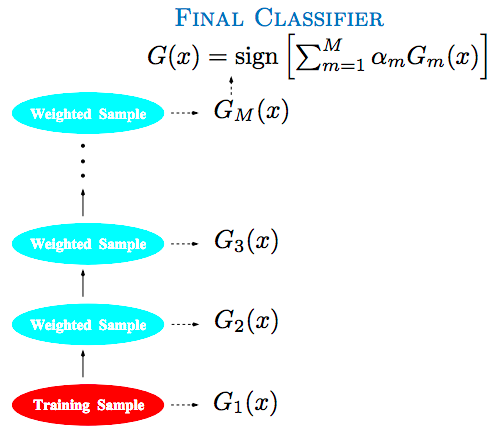
\includegraphics[height=0.7\textheight]{figures/adaboostSchematic}
\par\end{center}

\let\thefootnote\relax\footnotetext{\tiny{From ESL Figure 10.1}}
\end{frame}
%
\begin{frame}{AdaBoost - Rough Sketch}

\begin{itemize}
\item Training set $\cd=\left\{ \left(x_{1},y_{1}\right),\ldots,\left(x_{n},y_{n}\right)\right\} $.
\item Start with equal weight on all training points $w_{1}=\cdots=w_{n}=1$.
\item Repeat for $m=1,\ldots,M$:
\begin{itemize}
\item Base learner fits weighted training data and returns $G_{m}(x)$
\item Increase weight on the points $G_{m}(x)$ misclassifies 
\end{itemize}
\item Final prediction $G(x)=\sign\left[\sum_{m=1}^{M}\alpha_{m}G_{m}(x)\right]$.
(recall $G_{m}(x)\in\left\{ -1,1\right\} $)

\item What are desirable $\alpha_{m}$'s?
\pause
\begin{itemize}
\item nonnegative
\item larger when $G_{m}$ fits its weighted $\cd$ well
\item smaller when $G_{m}$ fits weighted $\cd$ less well
\end{itemize}
\end{itemize}

\end{frame}

%
\begin{frame}{Adaboost: Weighted Classification Error}
\begin{itemize}
\item Weights of base learners depend on their performance. How to evaluate each base learner?
\item In round $m$, base learner gets a weighted training set.
\begin{itemize}
\item Returns a base classifier $G_{m}(x)$ that minimizes weighted $0-1$
error.

\pause{}
\end{itemize}
\item The \textbf{weighted 0-1 error} of $G_{m}(x)$ is
\[
\mbox{err}_{m}=\frac{1}{W}\sum_{i=1}^{n}w_{i}\ind{y_{i}\neq G_{m}(x_{i})}\quad\text{where }W=\sum_{i=1}^{n}w_{i}.
\]

\item Notice: $\text{err}_{m}\in[0,1]$.
\end{itemize}
\end{frame}
%
\begin{frame}{AdaBoost: Classifier Weights}

\begin{itemize}
\item The weight of classifier $G_{m}(x)$ is $\alpha_{m}=\ln\left(\frac{1-\text{err}_{m}}{\text{err}_{m}}\right).$

\pause{}
\end{itemize}
\begin{center}
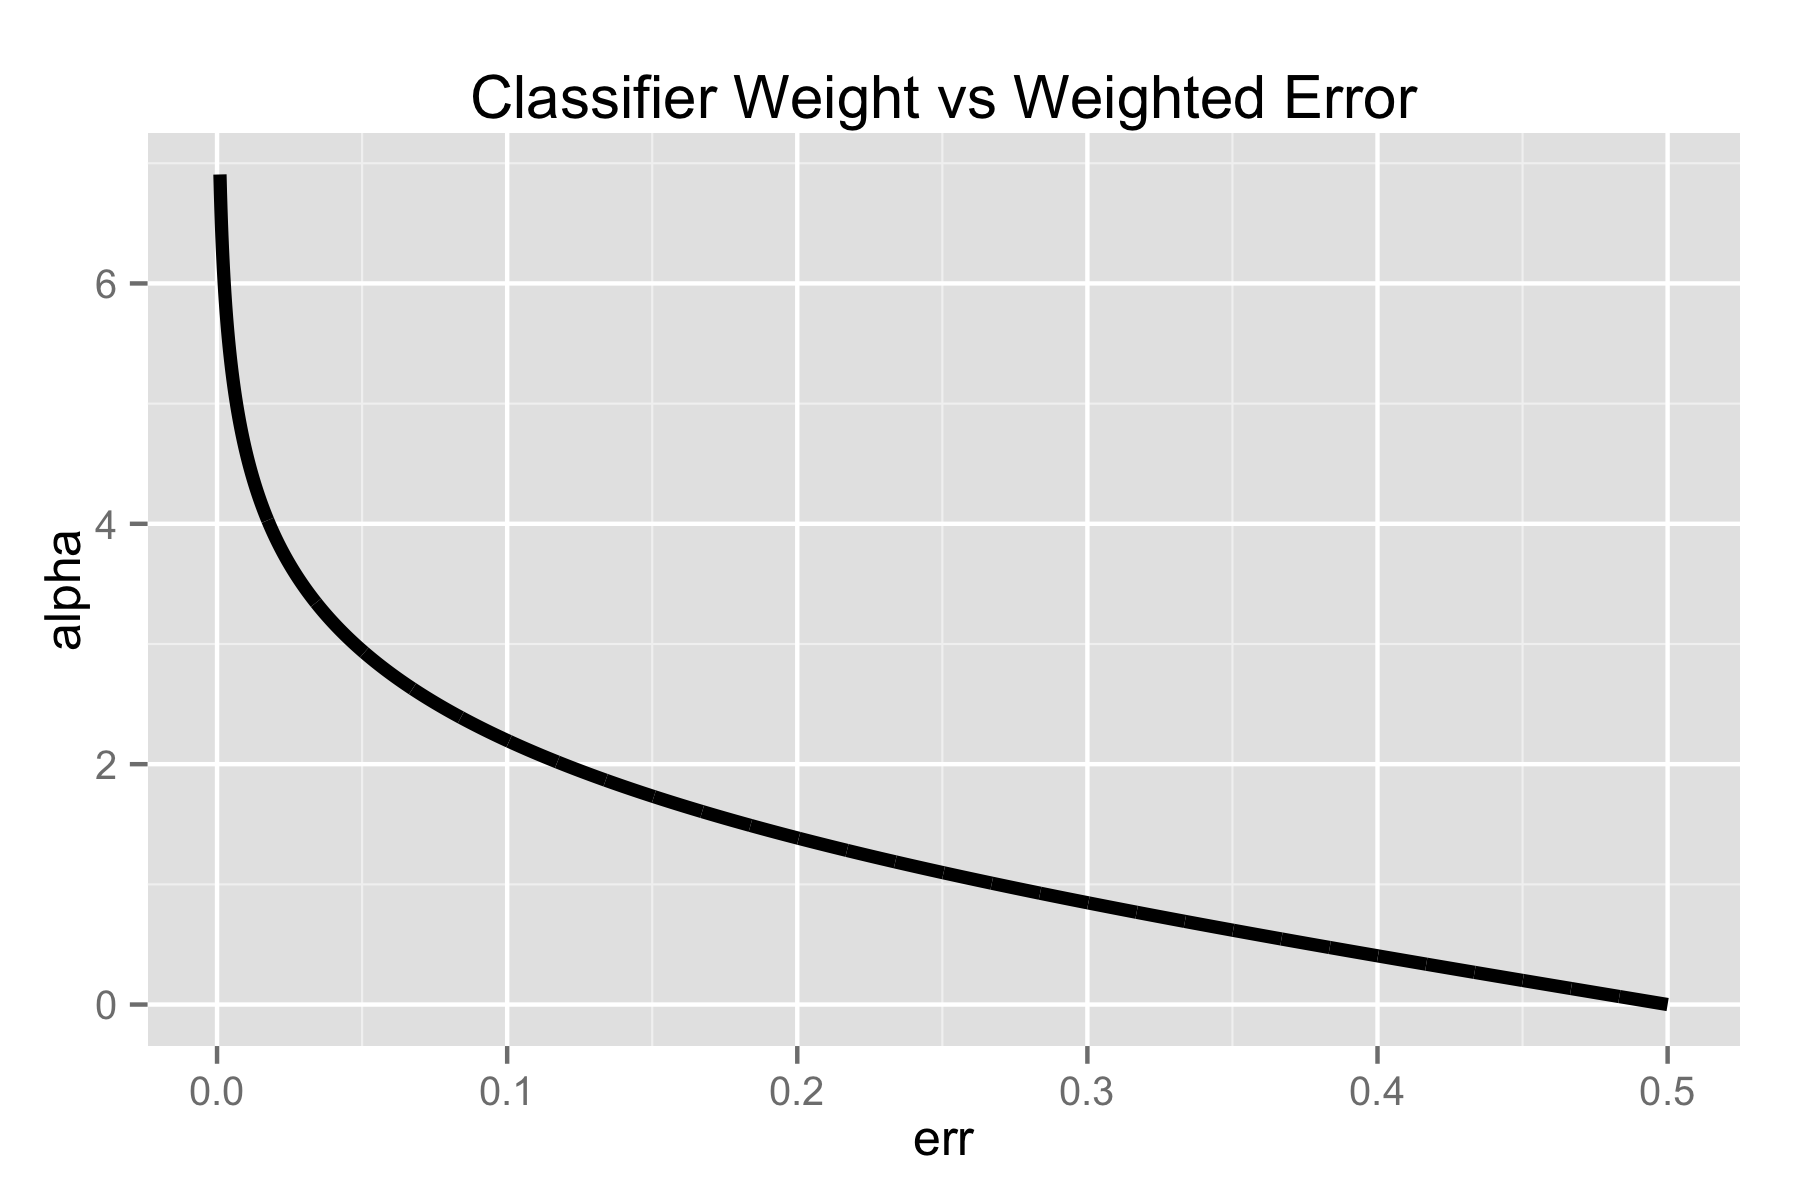
\includegraphics[clip,height=0.5\textheight]{figures/adaboostAlphaVsError}
\par\end{center}
\begin{itemize}
\item Higher weighted error $\implies$ lower weight
\item When is $\alpha_m < 0$?
\end{itemize}

\end{frame}
%
\begin{frame}{Adaboost: Example Reweighting}
\begin{itemize}
\item We train $G_{m}$ to minimize weighted error, and it achieves $\err_{m}$.

\item<.-> Then $\alpha_{m}=\ln\left(\frac{1-\text{err}_{m}}{\text{err}_{m}}\right)$
is the weight of $G_{m}$ in final ensemble.
\end{itemize}

\onslide<+->{
We want the base learner to focus more on examples misclassified by the previous learner.
}
\begin{itemize}[<+->]
\item Suppose $w_{i}$ is weight of example $i$ before training:
\begin{itemize}
\item If $G_{m}$ classfies $x_{i}$ correctly, then $w_{i}$ is unchanged.

\item Otherwise, $w_{i}$ is increased as 
\begin{eqnarray*}
w_{i} & \gets & w_{i}e^{\alpha_{m}}\\
& = & w_{i}\left(\frac{1-\text{err}_{m}}{\text{err}_{m}}\right)
\end{eqnarray*}

\item<.-> For $\mbox{err}_{m}<0.5$ (weak learner), this always increases the weight.
\end{itemize}
\end{itemize}
\end{frame}
%
%\begin{frame}{Adaboost: Example Reweighting}
%\begin{itemize}
%\item Any misclassified point has weight adjusted as $w_{i}\gets w_{i}\left(\frac{1-\text{err}_{m}}{\text{err}_{m}}\right)$.
%\end{itemize}
%\begin{center}
%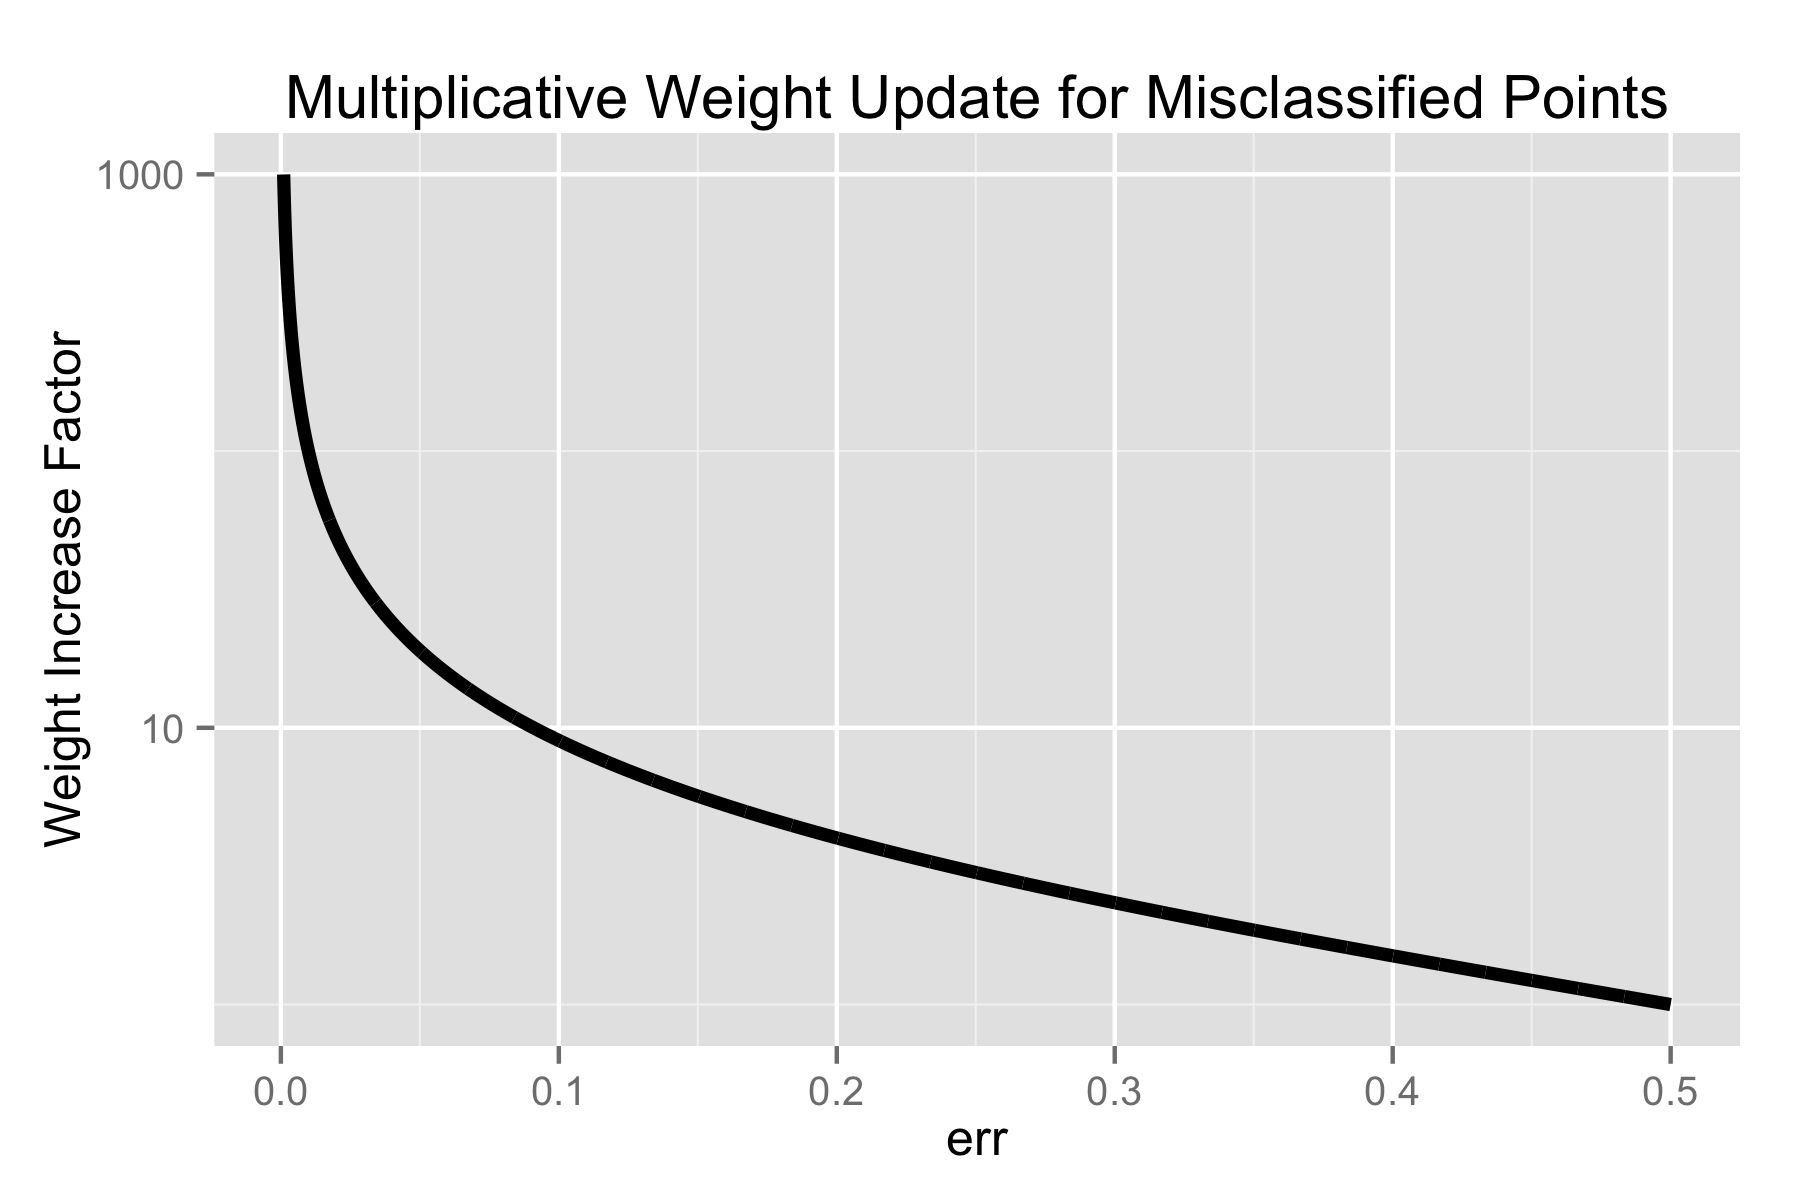
\includegraphics[clip,height=0.6\textheight]{figures/adaboostWeightUpdate}
%\par\end{center}
%\begin{itemize}
%\item The smaller $\err_{m}$, the more we increase weight of misclassified
%points.
%\end{itemize}
%\end{frame}
%
\begin{frame}{AdaBoost: Algorithm}

Given training set $\cd=\left\{ \left(x_{1},y_{1}\right),\ldots,\left(x_{n},y_{n}\right)\right\} $.
\begin{enumerate}
\item Initialize observation weights $w_{i}=1$, $i=1,2,\ldots,n$.

\pause{}
\item For $m=1$ to $M$:
\begin{enumerate}
\item Base learner fits weighted training data and returns $G_{m}(x)$

\pause{}
\item Compute \emph{weighted empirical 0-1 risk}:
\[
\mbox{err}_{m}=\frac{1}{W}\sum_{i=1}^{n}w_{i}\ind{y_{i}\neq G_{m}(x_{i})}\quad\text{where }W=\sum_{i=1}^{n}w_{i}.
\]


\pause{}
\item Compute  \emph{classifier weight}: $\alpha_{m}=\ln\left(\frac{1-\text{err}_{m}}{\text{err}_{m}}\right)$.

\pause{}
\item Update \emph{example weight}: $w_{i}\gets w_{i}\cdot\exp\left[\alpha_{m}\ind{y_{i}\neq G_{m}(x_{i})}\right]$

\pause{}
\end{enumerate}
\item Return \emph{voted classifier}: $G(x)=\sign\left[\sum_{m=1}^{M}\alpha_{m}G_{m}(x)\right]$.
\end{enumerate}
\end{frame}
%
\begin{frame}{AdaBoost with Decision Stumps}
\begin{itemize}
\item After 1 round:
\end{itemize}
\begin{figure}
\begin{centering}
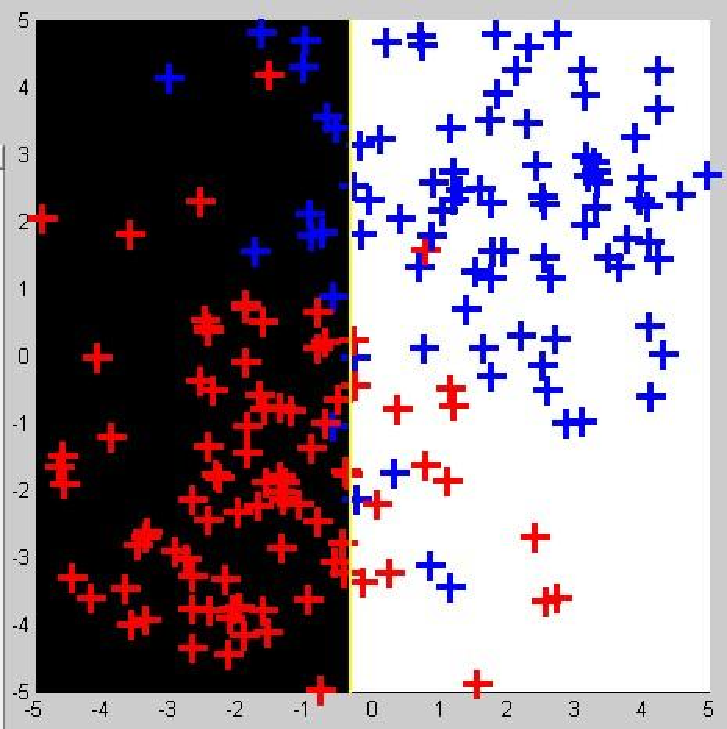
\includegraphics[height=0.5\textheight]{{figures/fig16.10a}.pdf}
\par\end{centering}
\caption{{\footnotesize{}Plus size represents weight. Blackness represents
score for red class.}}
\end{figure}

\let\thefootnote\relax\footnotetext{\tiny{KPM Figure 16.10}}
\end{frame}
%
\begin{frame}{AdaBoost with Decision Stumps}
\begin{itemize}
\item After 3 rounds:
\end{itemize}
\begin{figure}
\begin{centering}
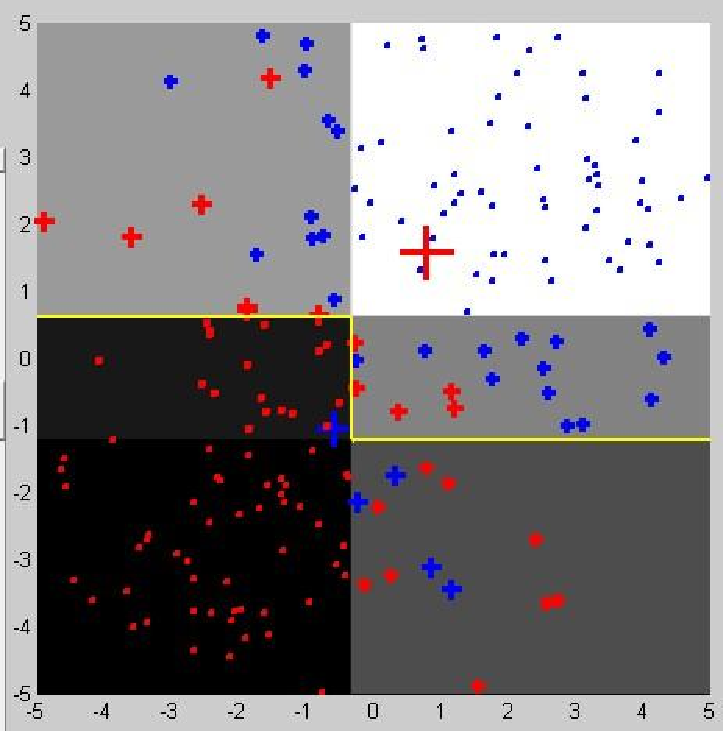
\includegraphics[clip,height=0.5\textheight]{{figures/fig16.10b}.pdf}
\par\end{centering}
\caption{{\footnotesize{}Plus size represents weight. Blackness represents
score for red class.}}
\end{figure}

\let\thefootnote\relax\footnotetext{\tiny{KPM Figure 16.10}}
\end{frame}
%
\begin{frame}{AdaBoost with Decision Stumps}
\begin{itemize}
\item After 120 rounds:
\end{itemize}
\begin{figure}
\begin{centering}
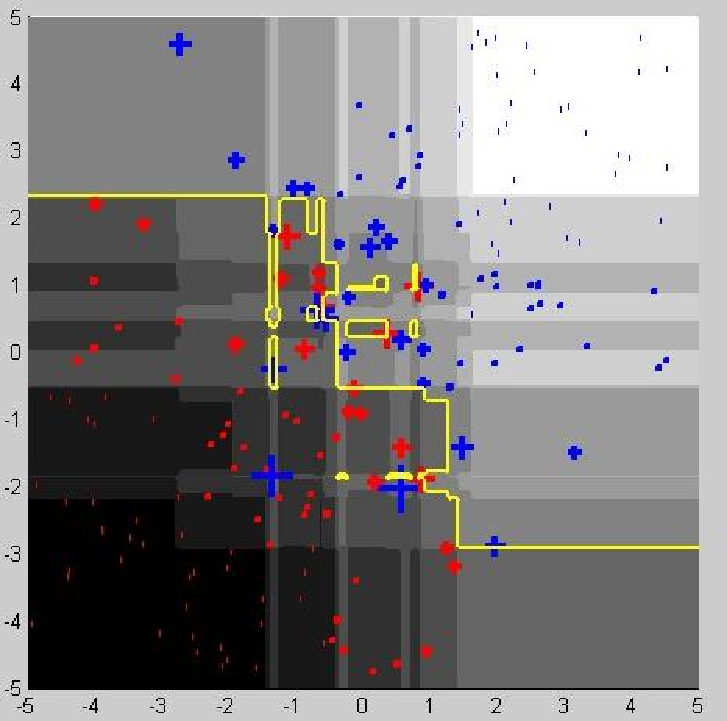
\includegraphics[height=0.5\textheight]{{figures/fig16.10c}.pdf}
\par\end{centering}
\caption{{\footnotesize{}Plus size represents weight. Blackness represents
score for red class.}}
\end{figure}

\let\thefootnote\relax\footnotetext{\tiny{KPM Figure 16.10}}
\end{frame}

\begin{frame}{Typical Train / Test Learning Curves}
\begin{itemize}
\item Might expect too many rounds of boosting to overfit:
\end{itemize}
\begin{center}
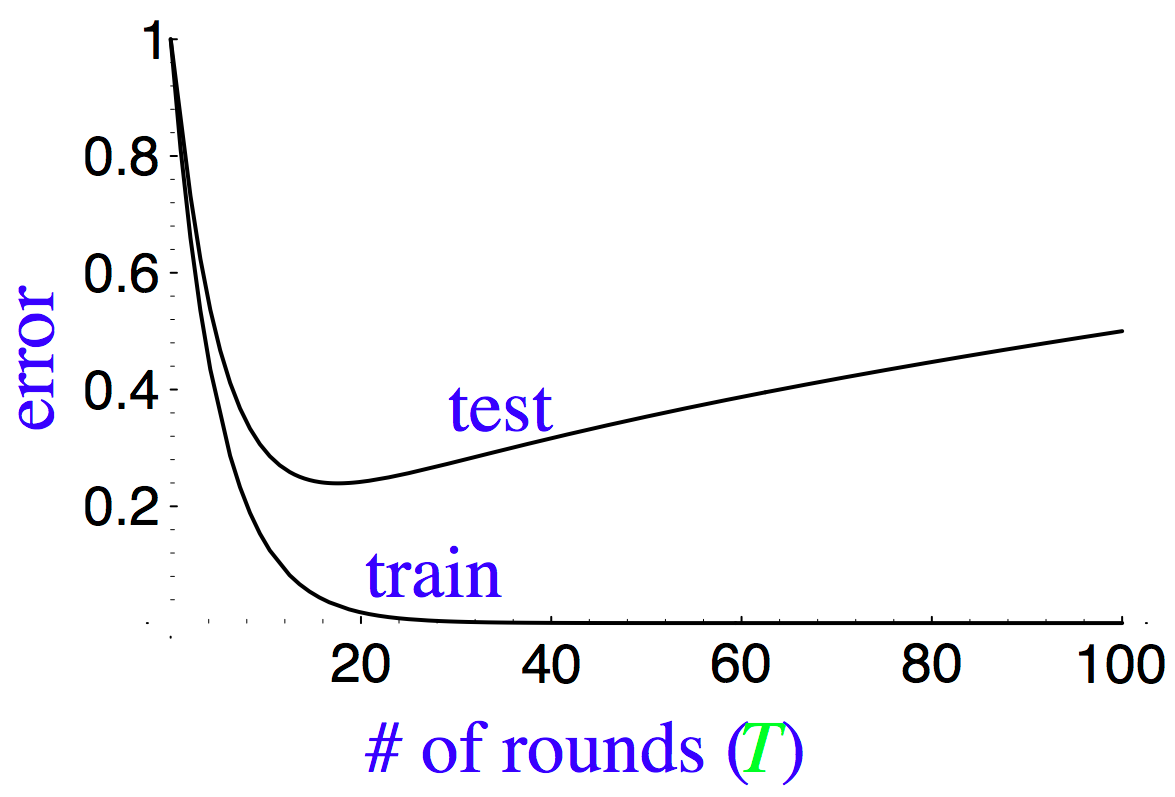
\includegraphics[height=0.65\textheight]{figures/typicalTrainTestCurve}
\par\end{center}

\let\thefootnote\relax\footnotetext{\tiny{From Rob Schapire's NIPS 2007 Boosting tutorial.}}
\end{frame}
%
\begin{frame}{Learning Curves for AdaBoost}
\begin{itemize}
\item In typical performance, AdaBoost is surprisingly resistant to overfitting.
\item Test continues to improve even after training error is zero!
\end{itemize}
\begin{center}
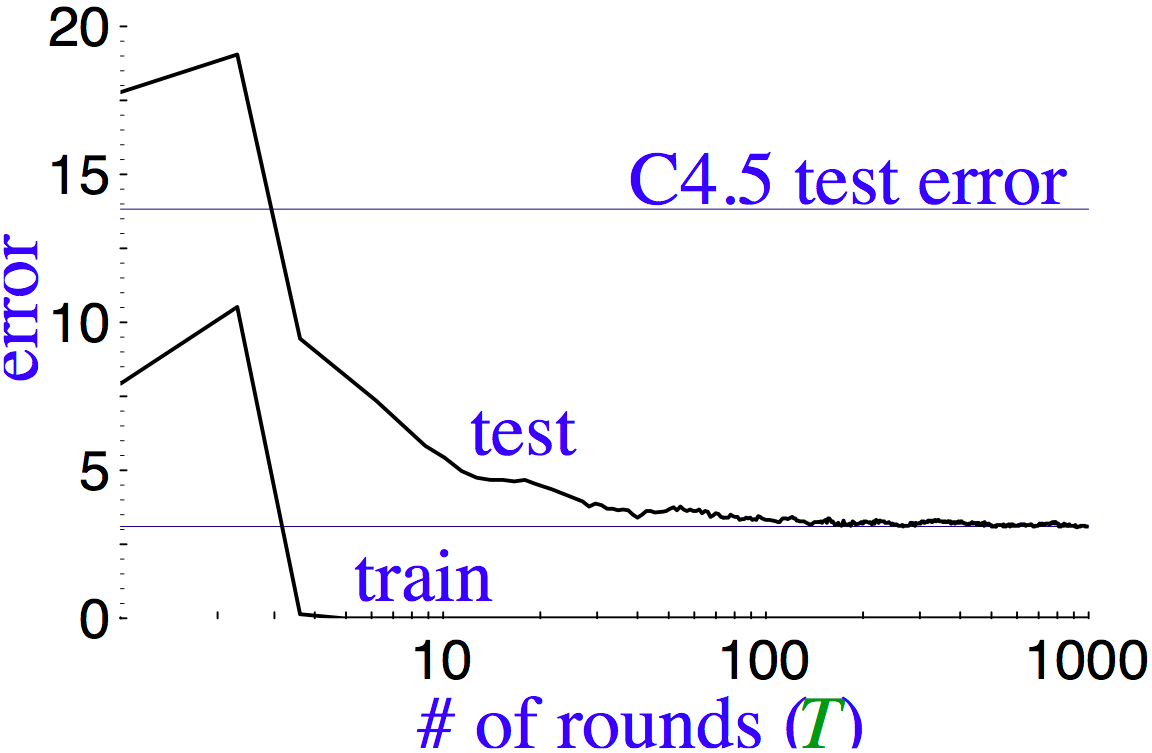
\includegraphics[height=0.65\textheight]{figures/actualTrainTestCurves}
\par\end{center}

\let\thefootnote\relax\footnotetext{\tiny{From Rob Schapire's NIPS 2007 Boosting tutorial.}}
\end{frame}


\begin{frame}
{Summary}
\begin{itemize}
\item Shallow decision tree + boosting
\begin{itemize}
\item ``best off-the-shelf classifier in the world''---Leo Brieman
\item Used in the first successful real-time face detector \href{https://www.cs.cmu.edu/~efros/courses/LBMV07/Papers/viola-cvpr-01.pdf}{(Viola and Jones, 2001)}
\item \href{https://xgboost.readthedocs.io/en/latest/index.html}{XGBoost}: very popular in competitions
\end{itemize}
\item Next week
\begin{itemize}
\item What is the objective function of Adaboost?
\item Generalize to other loss functions. 
\end{itemize}
\end{itemize}
\end{frame}

\end{document}
